\section{The Signal}\label{sec:signal}
In this thesis, I will compare \ac{ML} models in their ability to learn the trends of the data which will contribute  
in our ability separate the signal from the background. Specifically for this thesis, I will be studying an expansion of the 
\ac{SM} which includes super symmetry (see section \ref{subsec:SS}). The signal I will aim to separate from the background, is one 
which produces a WZ pair, through a neutralino and chargino pair. In figure \ref{fig:signal}, I have drawn a Feynman diagram for 
such a process. The Feynman diagram shows a neutralino and chargino pair, ($\tilde{\chi}_1$ and $\tilde{\chi}_2$)
where both sparticles produces a boson (W and Z respectively) and a $\tilde{\chi}_1$, the lightest neutralino. Given that the 
neutralinos in the final state are neutral, there are three leptons and a large amount of missing energy in the final state.
\begin{figure}
    \centering
    \makebox[0.75\linewidth][c]{%
    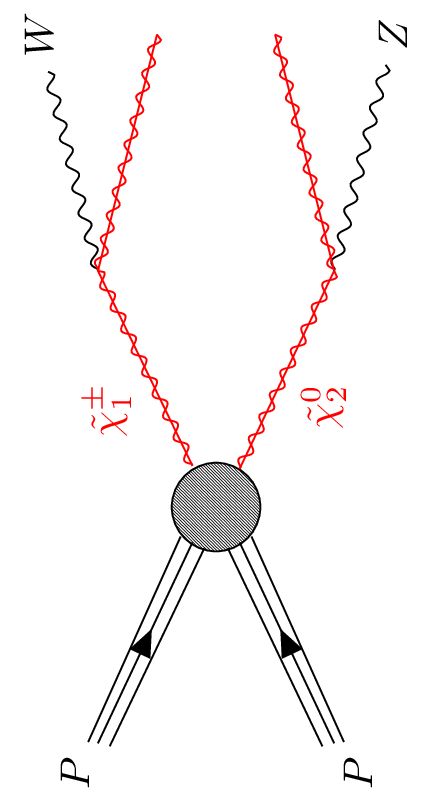
\includegraphics[width=0.225\textwidth, angle = -90]{Figures/FDiagrams/WZSignal.png}
    }
    \caption{The Feynman diagram of the signal-channel.}
    \label{fig:signal}
\end{figure}